\documentclass{article}

\def\changemargin#1#2{\list{}{\rightmargin#2\leftmargin#1}\item[]}
\let\endchangemargin=\endlist 

\usepackage[english]{babel}
\usepackage[utf8]{inputenc}
\usepackage{amsmath}
\usepackage{amssymb}
\usepackage{graphicx}
\usepackage{enumitem}
\graphicspath{{./images/}}
\usepackage{physics}
\usepackage{float}
\usepackage{multirow, array}
\usepackage[margin=140pt]{geometry}
\usepackage{tocloft}
\usepackage{dirtytalk}
\renewcommand{\cfttoctitlefont}{\hfill\Large\bfseries}
\renewcommand{\cftaftertoctitle}{\hfill\hfill}
\renewcommand{\cftloftitlefont}{\hfill\Large\bfseries}
\renewcommand{\cftafterloftitle}{\hfill}
\renewcommand{\cftlottitlefont}{\hfill\Large\bfseries}
\renewcommand{\cftafterlottitle}{\hfill}
% These 6 lines will center the titles of the table of contents, list of figures and list of tables
\newlist{notes}{enumerate}{1}
\setlist[notes]{label=Note: ,leftmargin=*}

\begin{document}

\begin{titlepage}
\pagenumbering{gobble}
\addcontentsline{toc}{section}{Abstract}
\begin{center}
\vspace{1cm}
\large
\textbf{Using Semialgebraic Parametric Analysis by Metaprogramming in Portfolio Optimization}

\normalsize
\vspace{.5cm}
Submitted as the Culmination of \\Undergraduate Research in Mathematics\\
\vspace{.5cm}
\textbf{Philip Meersman}\\
\vspace{.5cm}
\large
\vspace{.5cm}
\normalsize
\textbf{Abstract}
\end{center}
One classic problem in quantitative finance is portfolio optimization, which consists of assigning weights to assets in a portfolio to maximize one’s expected return while keeping the level of risk at a desired level. This problem can be modeled as a linear program (LP), using a risk aversion parameter mu. For a given single value of mu, the LP can be solved using any standard LP solver. In this work, however, the problem is considered parametrically: the optimal solution is sought for every possible value of mu. This describes how weights to the portfolio assets would be assigned from the timid investor to the bold. This is accomplished by applying the novel technique of semialgebraic parametric analysis by metaprogramming (SPAM). Demonstrated in this talk is the method of applying SPAM to a textbook example of portfolio optimization. Generated in this way are numerical and symbolic representations of the solution set as well as a graphical representation of these results.

\vfill
% \begin{figure}[H]
% \begin{center}
%\includegraphics[width=4cm]{err}
% \end{center}
% \end{figure}
\begin{center}	
University of Kentucky\\
College of Arts and Sciences\\
Bachelor of Science in Mathematics\\
Under the supervision of Dr. Yuan Zhou\\
May 2021\\
\end{center}
\end{titlepage}
\pagenumbering{gobble}
\tableofcontents
\pagebreak
\pagenumbering{gobble}
%\begin{center}\section*{Acknowledgments}\end{center}
%\addcontentsline{toc}{section}{Acknowledgments}
%appy Text

\pagebreak
\pagenumbering{arabic}
\section{Introduction}

Computer assistance in solving economic problems has recently become commonplace. In undergraduate economics courses students now learn to use Microsoft Excel, JMP, Stata, and other statistical software packages to expedite the once-tedious process of estimating regressions and computing variance, among other applications. One area of research benefiting from the propagation of computer programming is that of computer-assisted proofs. One such method of generating computer-assisted proofs is termed semialgebraic parametric analysis by metaprogramming (SPAM).

This paper first introduces a few toy examples demonstrating and describing the functionality of SPAM before illustrating its utility in two trivial applications from economics. Finally, the majority of the paper is spent discussing a more interesting economic application of SPAM: portfolio optimization. Note that we consider portfolio optimization in the context of Vanderbei's \textit{Linear Programming}.

While the topics in this paper are somewhat interesting and do demonstrate the capability of SPAM, they in no way attempt to capture its complete power. SageMath terminal and notebook output are provided in the Appendix, while certain useful figures are included throughout the paper.


\section{Traditional Portfolio Optimization}

One common undergraduate problem in financial economics is that of choosing weights to assign to assets in a portfolio to maximize one's expected return. In our experience this problem is first presented while involving two assets to choose from: one safe and one risky. The problem setup often specifies that the risky asset has a higher expected return than its safe counterpart, but with some non-zero probability may manifest a negative return. In solving problems of portfolio optimization it is important for one to keep in mind the type of problem they are solving. Depending on the formulation and desired format of solution, these problems can involve a variety of different variables, constraints, parameters, types of optimization, and conventions of notation. In this paper we use the framework detailed in Vanderbei [9], and specifically his section on the parametric simplex method. 

\subsection{Vanderbei's Formulation}
This simple formulation of the portfolio optimization problem naturally extends to the slightly more complicated problem of assigning weights to assets in a portfolio when each asset has its own, unique, expected value and unique level of risk. We consider a problem proposed by Vanderbei [9] in which nine risky assets are considered as possible portfolio pieces and their associated levels of risk are computed using historical data from 24 time periods. Historical data can be found in the Appendix. 

Adopting Vanderbei's notation, let the potential assets be indexed from $1$ to $n$ and let $R_j$ denote the return on investment $j$, with $j = 1,...,n$. Note that this $R_j$ is a random variable. A portfolio is comprised of a series of fractions of one's wealth that are assigned to some or all of the assets available. Let $x_j$ with $j = 1,...,n$ denote the fraction of one's wealth invested in asset $j$. Importantly, we must have that $\sum_{j=1}^{n} x_j = 1$. Then let the total return garnered by any given portfolio be:

\begin{center}
    $R = \sum_{j=1}^{n} x_jR_j$
\end{center}

While the reward associated with this portfolio is defined in terms of the expected return:

\begin{center}
    $\mathbf{E}(R) = \sum_{j=1}^{n} x_j\mathbf{E}(R_j)$
\end{center}

It is important to recognize the context of these portfolio optimization problems. For one, if the investor cares not about risk, then she will simply put all of her money into the asset with the highest expected return. This problem, while perhaps sometimes descriptive, is not interesting for use with SPAM. Instead, we consider a risk-averse decision maker. While there are several different interpretations and associated implications for what it means to measure risk aversion, we will adopt Vanderbei's basic metric: any number. Let $\mu \in [0,\infty)$ be one's level of risk aversion (their importance of risk relative to reward), with lower $\mu$ corresponding to a less risk-averse decision maker and higher $\mu$ corresponding to a more risk-loving decision maker. Intuitively, as $\mu$ approaches $\infty$ this problem becomes more and more similar to the problem involving someone who does not care at all about risk. In the case of extremely large $\mu$ the decision maker will choose the asset with the highest expected return. 

Just as there are many definitions of measures of risk-aversion, so too are there many definitions for risk itself. Vanderbei considers for this application the \textit{mean absolute deviation from the mean (MAD)} as a definition for risk:

\begin{center}
    $\mathbf{E}\abs{(R - \mathbf{E}(R))} = \mathbf{E}(\abs{\sum_{j=1}^{n} x_j(R_j-\mathbf{E}(R_j)})$
\end{center}

Now having a measure of risk to consider, we are interested in the individual trying to maximize expected return subject to whatever constraint their level of risk aversion imposes on them. Risk and reward can be combined with the risk aversion parameter $\mu$ to produce:

\begin{center}
    $\zeta = \mu\sum_{j} x_j\mathbf{E}(R_j) - \mathbf{E}(\abs{\sum_{j} x_j(R_j-\mathbf{E}(R_j)))}$
\end{center}

This defines the decision maker's objective function, valuing reward and disliking risk. Notice that as $\mu$ tends toward $\infty$ the positive reward term will dominate the negative risk term, consistent with the description above. 

\begin{notes}
\item In this chapter Vanderbei briefly describes the \textit{hedging} process. For our purposes, hedging can simply be thought of as reducing risk without reducing expected reward, and if such an opportunity exists one should take it. This obviously has many extensions in financial economics but is not a focus of our work.
\end{notes}

In order to evaluate $\zeta$ it appears one must know the joint distribution of the $R_j$'s. While this could be given as part of a problem's description, generally distributions of financial data are not known with certainty, but can be estimated using historical financial data. This is what Vanderbei does. The following table describes historical data for nine different assets over 24 one-month periods. This data will be used to estimate the expected returns of each asset for the purposes of portfolio optimization.

TABLE?

Now, let $R_j(t)$ be the return on investment $j$ during time period $t$ with $t \in T = \{1,2,...,24\}$. Using the average of the historical returns for each asset, the expected return for each is denoted:

\begin{center}
    $\mathbf{E}(R_j) = \frac{1}{T}\sum_{t=1}^{T} R_j(t)$
\end{center}

This problem can be compiled to the form:

\begin{align*}
&\text{maximize}  &&\text{$\mu\sum_{j} x_jr_j - \frac{1}{T}\sum_{t=1}^{T}\abs{\sum_{j} x_j(R_j(t)-r_j)}$}\\
&\text{such that}  &&\text{$\sum_{j} x_j = 1$}\\
&\text{}  &&\text{$x_j \geq 0$ \hspace{10pt} $j = 1,2,...,n$}
\end{align*}

with

\vspace{5pt}
\begin{center}
    $r_j = \frac{1}{T}\sum_{t=1}^{T} R_j(t)$
\end{center}
\vspace{5pt}

This problem includes several absolute values in the objective function, which are inconvenient. In order to work around this, Vanderbei introduces a new variable, $y_t$, to replace each absolute value. By imposing new inequality constraints on $y_t$, the absolute values can be accurately represented in the linear program. As stated, replace $\abs{\sum_{j} x_j(R_j(t)-r_j)}$ with $y_t$ to obtain our problem as

\begin{align*}
&\text{maximize}  &&\text{$\mu\sum_{j} x_jr_j - \frac{1}{T}\sum_{t=1}^{T} y_t$}\\
&\text{such that}  &&\text{$\sum_{j} x_j = 1$}\\
&\text{}  &&\text{$-y_t \leq \sum_{j} x_j(R_j(t)-r_j) \leq y_t \hspace{20pt} t = 1,2,...,T$}\\
&\text{}  &&\text{$y_t \geq 0$ \hspace{10pt} $j = 1,2,...,n$}\\
&\text{}  &&\text{$x_j \geq 0$ \hspace{9pt} $j = 1,2,...,n$}
\end{align*}

This problem can be solved for any desired value of $\mu$. However, we have tools to systematically solve this parametric linear program for \textit{every} value of $\mu$ using the parametric simplex method. This is the manual process that SPAM expedites and automates.

\begin{notes}
\item In this context, a problem of portfolio optimization is defined by the number of assets available, their historical data, and $\mu$. This is all that is necessary to define such a problem.
\end{notes}

\subsection{Parametric Simplex Method}

To use the parametric simplex method, one must choose a starting value of the parameter. It is desirable to choose a value for $\mu$ that results in an "obvious" basic optimal solution. If this is possible we can then begin experimenting with changes in the parameter value. In the case of a portfolio optimization problem, it is natural to choose a value for $\mu$ that will result in $x_j^* = 1$ (if possible) where $j^*$ is the asset with highest expected return. To perform the parametric simplex method Vanderbei introduces slack variables $w_t^+$ and $w_t^-$ and rewrites the problem in dictionary form:

\begin{align*}
&\text{maximize}  &&\text{$\mu\sum_{j} x_jr_j - \frac{1}{T}\sum_{t=1}^{T} y_t$}\\
&\text{such that}  &&\text{$-y_t - \sum_{j} x_j(R_j(t)-r_j)+w_t^- = 0$}\\
&\text{}  &&\text{$-y_t + \sum_{j} x_j(R_j(t)-r_j)+w_t^+ = 0$}\\
&\text{}  &&\text{$\sum_{j} x_j = 1$}\\
&\text{}  &&\text{$y_t \geq 0$ \hspace{10pt} $j = 1,2,...,n$}\\
&\text{}  &&\text{$x_j \geq 0$ \hspace{9pt} $j = 1,2,...,n$}
\end{align*}

Still assuming that we have chosen $\mu$ such that $x_j^* = 1$, the other $x_j$'s disappear. Remaining variables that are positive are considered basic and the rest are considered nonbasic. So, $x_j^*$ is basic, while the rest of the $x_j$'s are nonbasic. Also, $y_t$'s are nonzero and thus basic. For each $t$, one of $w_t^+$ or $w_t^-$ is basic while its counterpart is nonbasic. To state which is basic, Vanderbei introduces some more notation. Let

\begin{center}
    $D_t_j = R_j(t) - r_j$
\end{center}

Then if $D_t_j^* > 0$, $w_t^-$ is basic. If $D_t_j^* < 0$, $w_t^+$ is basic. If it occurs that $D_t_j^* = 0$, one can arbitrarily decide while of the $w_t$ is basic. Let

\begin{center}
    $T^+ = \Bigg\{t: D_t_j^* > 0\}$ and $T^- = \{t: D_t_j^* < 0\}$
\end{center}

and 

\begin{center}
    $\epsilon_t = \{1$ for $t\in T^+$ \\
    $\epsilon_t = \{-1$ for $t\in T^-$
\end{center}

Then after solving this via parametric simplex method, the optimal dictionary is: \\

$\zeta = \frac{1}{T}\sum_{t=1}^{T}\epsilon_tD_t_j^*-\frac{1}{T}\sum_{j\ne j^*} \sum_{t=1}^{T} \epsilon_t(D_t_j-D_t_j^*)x_j\\ \\ -\frac{1}{T}\sum_{t\in T^-} w_t^- -\frac{1}{T}\sum_{t\in T^+} w_t^+ + \mu r_j^* + \mu \sum_{j\ne j^*} (r_j - r_j^*)x_j$

\begin{center}
    \rule{\textwidth}{0.4pt}
\end{center}
with
\begin{align*}
&\text{$y_t$}  &&\text{=} &&&\text{$-D_t_j^*$} &&&&\text{$-$} &&&&&\text{$\sum_{j\ne j^*} (D_t_j-D_t_j*)x_j$} &&&&&&\text{$+w_t^-$} &&&&&&&\text{} &&&&&&&&\text{$t \in T^-$}\\
&\text{$w_t^-$}  &&\text{=} &&&\text{$2D_t_j^*$} &&&&\text{$+$} &&&&&\text{$2\sum_{j\ne j^*} (D_t_j-D_t_j*)x_j$} &&&&&&\text{} &&&&&&&\text{$+w_t^+$} &&&&&&&&\text{$t \in T^-$}\\
&\text{$y_t$}  &&\text{=} &&&\text{$D_t_j^*$} &&&&\text{$+$} &&&&&\text{$\sum_{j\ne j^*} (D_t_j-D_t_j*)x_j$} &&&&&&\text{} &&&&&&&\text{$+w_t^+$} &&&&&&&&\text{$t \in T^-$}\\
&\text{$w_t^+$}  &&\text{=} &&&\text{$-2D_t_j^*$} &&&&\text{$-$} &&&&&\text{$2\sum_{j\ne j^*} (D_t_j-D_t_j*)x_j$} &&&&&&\text{$+w_t^-$} &&&&&&&\text{} &&&&&&&&\text{$t \in T^-$}\\
&\text{$x_j^*$}  &&\text{=} &&&\text{1} &&&&\text{$-$} &&&&&\text{$\sum_{j\ne j*} x_j$} &&&&&&\text{} &&&&&&&\text{} &&&&&&&&\text{}
\end{align*}
\\
\\

For large values of $\mu$, it is easy to check that this dictionary is optimal. The objective coefficients on $w_t^-$ and $w_t^+$ in the objective function are both negative. Coefficients on $x_j$'s in the first row of the objective function can be positive or negative depending on the differences $D_t_j - D_t_j^*$, but for a $\mu$ large enough, the coefficients on $x_j$'s in the second row will grow dominant over the first row coefficients. This forces the coefficients on $x_j$'s negative. From Vanderbei's definition of $T^-$ and $T^+$, all basic variables here are positive. 

Notice that as $\mu$ is allowed to vary (decrease, in this case) the coefficients on some $x_j$'s will eventually become zero and then positive. As this happens, the parametric simplex method sends the $x_j$ corresponding to the now-positive coefficient into the basis. As usual, the ratio test is conducted on coefficients containing $\mu$ in the old dictionary to determine which variable will leave the basis. Once this pivot has been performed, we are left with a new dictionary corresponding to a new value of $\mu$. The $\mu$ value for which one coefficient on the $x_j$'s changes from negative to positive is a possible boundary value for $\mu$ at which the objective value (and hence optimal solution to the linear program) changes. This process can be repeated as many times as necessary until $\mu$ becomes 0. In general, the parametric simplex method is not bounded by a parameter value of 0, but in this case of portfolio optimization $\mu < 0$ does not make sense.

After performing the parametric simplex method to completion, one has a series of $\mu$\textit{-intervals}. Each $\mu$-interval is bounded by values of $\mu$ for which the objective function value changes. Within any given $\mu$-interval, any value of $\mu$ will result in the same objective value and optimal solution. This is the result of the parametric simplex method. In the (still generalized) case of portfolio optimization, one also obtains the objective value and associated optimal solution for each $\mu$-interval. If thought of as percentages, the $x_j$'s can be plotted against the list of $\mu$-intervals to produce an \textit{efficient frontier} for any given problem. This efficient frontier is what is "rediscovered" using SPAM.

\section{SageMath}

Now that Vanderbei's method is understood, we will introduce our work with SPAM and the problem of portfolio optimization. Just as any problem must be translated from plain text to function in a programming language, so too must our problem. Personally, I began this project with little knowledge of Python and no knowledge of SageMath, so there was much time spent familiarizing ourselves with the two. Many unforeseen technical obstacles surfaced throughout this process, and I describe them here chronologically.

\subsection{SageMath Setup}

For our project we used SageMath from source (various versions between 8.9 and 9.3.beta6) via Ubuntu on the Windows Subsystem for Linux. We used SageMath both in terminal and in Jupyter notebook. Most of our work in the terminal was done by loading .sage files from our local machine to the terminal each session. We saved output often as .txt files and stored them locally. Work in notebooks was also done using .ipynb files saved locally. In most cases we pushed/pulled changes using GitHub Desktop, although we did also use git version control from the Linux terminal (this was necessary to pull ticket changes from SageTrac before they were published in a stable release of SageMath). While I did attempt to work on SageMath development, I found this less interesting and more alien than using SageMath, so most of our time was spent working with the software. 

\subsection{SPAM}

Originally developed to automate the discovery of new 
cut-generating functions in linear programming [.], 
SPAM is an algorithm applied to an existing program, $P$, which exhibits certain nice properties. Without a standalone program to feed as input into SPAM, it does nothing on its own.

\subsection{Requisite Properties of $P$} 
First, the mathematical problem being solved by $P$ must be parameterized. One or more parameters of interest must appear in $P$, otherwise $P$ simply solves one concrete problem and there is nothing interesting to be gained from SPAM. The parameters are often grouped in a fixed tuple, $\sigma$. These parameters are explicitly declared as elements of a Parametric Real Field, $K$. Creating such a field indicates to SPAM which parameters to recognize throughout the execution of $P$. 

Second, $P$ must rely only on algebraic operations, branches, and comparisons. Specifically, the algebraic operations conducive for use with SPAM are elementary algebraic operations on real numbers. Branches allowed are traditional if-then-else statements and loops. These properties ensure that the set of parameters where SPAM returns any particular outcome is a semialgebraic set. This is necessary for SPAM, and rules out programs relying on more sophisticated operations. 

Also important to note, SPAM is formatted for Python, and specifically within the SageMath computer algebra software [1]. Naturally, programs we discuss and introduce are written in Python and are all executed in SageMath. This paper contains a combination of programs previously existing in Python libraries, programs written by Dr. Zhou, and programs written by myself. 

In short, there are three components required for an effective use of the SPAM algorithm.
\begin{enumerate}
    \item A program (algorithm) which acts on a parameter tuple, $P(\sigma)$
    \item A proof cell generated by metaprogramming, $SPAM(P(\sigma))$
    \item A \textit{proof cell complex} combining every proof cell generated by the SPAM algorithm, $SPAM^*(P)$
\end{enumerate}

In short, this constitutes the process of using SPAM by applying it to an existing Python program. The result can vary from problem to problem, but is usually depicted in graphical form in some capacity. Since SPAM records comparisons in the form of inequalities, it is natural to plot those inequalities to separate proof cells by output value. 

\begin{notes}
\item In order to use SPAM to generate precise inequality comparisons, we use rational-valued numbers in computation. Because of the approximation involved in computing with floating point numbers, rationals are more appropriate for SPAM. We refer to numbers used within our programs in fractional form.
\end{notes}

\subsection{Example: Positive Definite Matrix}

Consider a program $P$ which takes a matrix as input and yields as output a Boolean True if the matrix is positive definite and False otherwise. In Python this program is actually the {\fontfamily{qbk}\selectfont is\_positive\_definite} method from class \textit{Matrix}. This is a very elementary program but does well to illustrate the use of SPAM without having to digest mathematics simultaneously. Consider the matrix
\bigskip
\linebreak
\bigskip
\centerline{$A = $ \begin{bmatrix} \frac{1}{3} & a\\ a & b \end{bmatrix}}

One may ask the question \say{For which values $(a,b)$ is this matrix positive definite?} 
In this example one can compute the principal minor of $A$ and generate an inequality solution to this question by hand. Since this is not a complicated question, one might suggest an answer in the form of a theorem. Theorem 1: $A$ is positive definite if and only if the following holds
\bigskip
\linebreak
\bigskip
\centerline{$\frac{b}{3} - a^2 > 0$}

We now hope that SPAM can provide some sort of proof of this theorem. To accomplish this, we can use {\fontfamily{qbk}\selectfont is\_positive\_definite}, as it relies only on algebraic operations and is parameterized here by $(a,b)$. In handling each iteration of {\fontfamily{qbk}\selectfont is\_positive\_definite}, recall that SPAM records both numerical comparisons (which are generally unseen by the user) as well as the associated symbolic representation of each inequality along the way. These will become the basis for our proof cell complex.

A complete proof cell will contain, at minimum, a list of symbolic expressions corresponding to the inequalities recorded during the execution of $P$ and an optimal solution value corresponding to every parameter value within the proof cell. In Figure 1 each proof cell is distinguished in color by the output of $P$ when given parameter tuple $(a,b)$ with a concrete value. Red cells correspond to matrices that are not positive definite ($P$ output False) while blue cells correspond to matrices that are positive definite ($P$ output True).

\vspace{20pt}

\begin{center}
    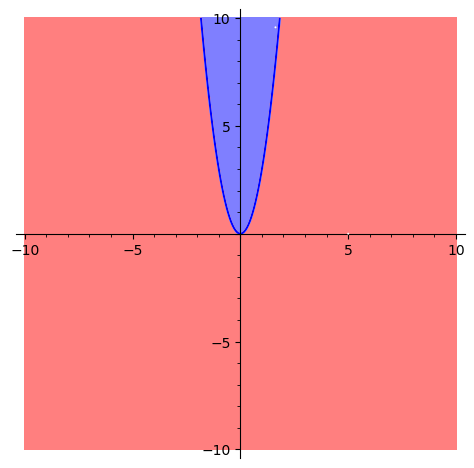
\includegraphics[width=6cm]{posdef_graph.png} \\
    \caption{The proof cell complex associated with matrix $A$ and {\fontfamily{qbk}\selectfont is\_positive\_definite.}}
\end{center}
\vspace{20pt}

In this case, the proof cell complex shows all combinations of parameter values that result in a positive definite matrix. This \say{proves} Theorem 1. So, the usefulness of SPAM here is in creating a comprehensive solution to the parametric problem characterized by the matrix $A$. The two small white dots (one in the blue region and one in the red) indicate the test points that were used by SPAM to generate their cells. Instead of having to solve this problem for the infinitely many values of $(a,b)$, one can employ SPAM to generate this proof cell complex describing the solution for \textit{every} tuple of parameter values. This is the value SPAM adds, an algorithm that provides complete solutions to parameterized problems. 

\subsection{Example: Reducing System of Inequalities}

Once we understood the basic principle of SPAM, we looked for possible applications in economics. My first attempt in applying SPAM to an economic problem was in reducing a redundant system of inequalities generated by a game of Cournot competition. 

The classical two-player game modeling the actions taken between members of a duopoly is solved by obtaining a Nash-Cournot equilibrium. Specifically, this analysis is focused on the old problem concerned with finding optimal levels of research and development in a two-firm setting. This is achieved with restrictions on the five parameters (a, A, $\beta$, b, $\gamma$) within the d'Aspremont-Jacquemin duopoly model [3]. In their paper three different scenarios are presented, with three different sets of inequalities bounding the parameters. We will focus on their first example here. Six inequalities constitute these restrictions, and are summarized here for reference:
\begin{enumerate}
\item$0 < A < a$
\item$0 < \beta < 1$
\item$\frac{(a - A)(2 - \beta)}{4.5b\gamma - (2-\beta)(1+\beta)} > 0$
\item$\frac{2(a-A)(4.5b\gamma)}{3b(4.5b\gamma-(2-\beta)(1+\beta))}>0$
\item$\frac{(a-A)(2-\beta)(1+\beta)}{4.5b\gamma-(2-\beta)(1+\beta)}<A$
\item$\frac{2}{9}(2-\beta)^{2}<b\gamma$
\end{enumerate}

If this system is satisfied by values of all five parameters, then the optimal level of research and development as well as the optimal level of profit have meaningful values in this problem. These are enumerated explicitly by d'Aspremont and Jacquemin.

In order to utilize SPAM, one must create (or obtain) a "point-wise prover" program. This program must only function using semialgebraic operations in order to remain suitable for SPAM. For this application, we created a point-wise prover of our own, dubbed "ineq2" [3]. Ineq2 is a simple program designed to test values for each of the five parameters of interest and then return True if the system of inequalities is satisfied and return False if they are not. This simple operation of checking inequalities preserves the desired properties of a semialgebraic solution set.

Once verifying this program's validity, we used it as an input for SPAM. This process involves giving ineq a concrete set of arguments to pass. In our case, we chose to use $(a, b, A, \beta, \gamma)=(2, 1, 1, 1/2, 10)$ as the starting point for SPAM. All of our analysis takes place in the five-dimensional parameter space. We chose these parameter values because they yield a result of True when passed through ineq and thus satisfy the original set of inequalities from above.

Once SPAM has this concrete-valued tuple it begins its work. We used the breadth-first search (BFS) method from SPAM. With this method, the BFS first executes ineq with the given tuple and records both the Boolean result from ineq as well as the inequalities that are checked. This data is stored in a proof cell by SPAM and eventually constitutes one cell of the complex. Once BFS completion is achieved, analysis of the proof cell complex can begin. In this paper, the description of a proof cell is identical to the set of inequalities which define it, and vice versa.

Upon BFS completion a proof cell complex is yielded. This complex of cells defined by sets of inequalities lives in the parameter space, and each cell is either defined as "True" or "False", depending on the return value from ineq when components of those cells are passed through. In this case five proof cells are generated. One of these cells is "True". This is the cell we are interested in, we will refer to it as "Cell 0".

It is simple enough, once SPAM has finished its work, to access the data stored for each cell in the complex. Cell 0 is described by a system of inequalities, which are listed here:
\begin{enumerate}
\item$0 < \gamma$
\item$0 < \beta < 1$
\item$0 < A < a$
\item$0 < b$
\item$-2\beta^{2} - 9b\gamma + 2\beta + 4 < 0$
\item$2\beta^{2} - 9b\gamma - 8\beta + 8 < 0$
\item$-2a\beta^{2} -9bA\gamma + 2a\beta +4a < 0$
\end{enumerate}

We were cautious to accept that these two sets of inequalities were equivalent. After all, there are additional linear inequalities as well as one fewer high-degree inequality in this cell than in the original one. To test for equivalency of these two cells we first created a separate program designed to check this, called "ineq\_check". As before, let our new set of inequalities be "Cell 0" and the original set be "Cell 1". Ineq\_check works in the following way:
\begin{enumerate}
    \item Generate a tuple in the parameter space with random values for each parameter.
    \item Initialize a list to store truth values for each execution.
    \item Check this newly generated tuple for membership in Cell 1.
    \item Check again for membership in Cell 0. 
    \item If this tuple is a member of Cell 1 and Cell 0 add "True" to the list.
    \item If this tuple is \emph{not} in Cell 1 and also \emph{not} in Cell 0, add "True" to the list.
    \item If this tuple is a member of one cell but not the other, add "False" to the list.
    \item Repeat the above steps 100,000 times.
    \item Check the list for any instances of "False". Return False if so.
    \item If no instances of "False" in the list, return True.
\end{enumerate}

After running this program many times and getting a result of True every time, we began to suspect the two cells were identical. Every point we had randomly generated and tested was either contained in both cells or neither cell. We suspected that, with some algebra and rearranging of terms, the following inequalities are implied between the two cells. Inequalities (5), (6), and (7) from Cell 0 are the same as inequalities (4), (6), and (5) from Cell 1:

\begin{eqnarray}
-2\beta^{2} - 9b\gamma + 2\beta + 4 < 0 &\equiv& \frac{2(a-A)(4.5b\gamma)}{3b(4.5b\gamma-(2-\beta)(1+\beta))}>0\\
2\beta^{2} - 9b\gamma - 8\beta + 8 < 0 &\equiv& \frac{2}{9}(2-\beta)^{2}<b\gamma\\
-2a\beta^{2} -9bA\gamma + 2a\beta +4a < 0 &\equiv& \frac{(a-A)(2-\beta)(1+\beta)}{4.5b\gamma-(2-\beta)(1+\beta)}<A
\end{eqnarray}

In some sense, Cell 0 is a \say{simpler} description of the original set of inequalities. It contains one fewer high-degree inequality. However, Cell 0 does impose new constraints on $\gamma$ and b. This is the trade-off. In using this method for reducing systems of inequalities, one must decide whether they desire fewer high-degree inequalities or fewer total inequalities. In either case, this project has provided an alternative description of the set of inequalities bounding the parameters in d'Aspremont and Jacquemin's analysis of two-firm games.

\section{Rediscovery of Textbook Results}

\subsection{Demonstration on Small Dataset}

Prior to discussing the results from the full nine-asset 24-period problem that Vanderbei uses, we introduce a small three-asset two-period model for demonstration. Consider \say{historical data}:


\begin{center} 
\begin{tabular}{ |c|c|c|c| } 
\hline
Time period & j=1 & j=2 & j=3 \\
\hline
1 & $\frac{5}{3}$ & $\frac{7}{3}$ & 1 \\[10pt]
2 & $\frac{2}{3}$ & $\frac{1}{3}$ & $\frac{3}{4}$\\
\hline
\end{tabular}
\end{center}

This data can also be represented as a triplet of tuples

\begin{center}
    $((\frac{5}{3}, \frac{2}{3}), (\frac{7}{3}, \frac{1}{3}), (1,\frac{3}{4}))$
\end{center}

with each tuple representing the historical returns for its associated asset. Using dictionary notation and combining coefficients on like terms, this example can be formatted as a linear program:

\begin{align*}
&\text {} &&\text{maximize}  &&&\text{$\frac{7}{6}\mu x_1 + \frac{4}{3}\mu x_2 + \frac{7}{8}\mu x_3 - \frac{1}{2} x_4 - \frac{1}{2}x_5$}\\
\\
&\text{}&&\text{such that}  &&&\text{$\frac{1}{2}x_1 + x_2 +  \frac{1}{8}x_3 - x_4 \leq 0$}\\
&\text{}&&\text{}  &&&\text{$-\frac{1}{2}x_1 - x_2 -  \frac{1}{8}x_3 - x_4 \leq 0$}\\
&\text{$LP $ = }&&\text{}  &&&\text{$-\frac{1}{2}x_1 - x_2 -  \frac{1}{8}x_3 - x_5 \leq 0$}\\
&\text{}&&\text{}  &&&\text{$\frac{1}{2}x_1 + x_2 +  \frac{1}{8}x_3 - x_5 \leq 0$}\\
&\text{}&&\text{}  &&&\text{$x_1 + x_2 + x_3 = 1$}\\
&\text{}&&\text{}  &&&\text{$x_j \geq 0$ \hspace{9pt} $j = 1,2,3$}
\end{align*}
\\

Where $x_1, x_2, x_3$ are weights on assets 1, 2, 3, respectively and $x_4, x_5$ are variables representing the absolute value terms mentioned earlier. The linear program is not explicitly set up with slack variables included, those are added by the SageMath solver when the program is solved. We wrote a program {\fontfamily{qbk}\selectfont setup\_portfolio\_lp} which takes, as input, a tuple containing historical data and a value for $\mu$, which together define a portfolio optimization problem.

For example, this is the SageMath command and output when\\ {\fontfamily{qbk}\selectfont setup\_portfolio\_lp} is called on this small example with $\mu = 5$:

%fix this Sage command formatting
\begin{align*}

&\text{}
&\text{sage: hist\_data = $((\frac{5}{3},\frac{2}{3}),(\frac{7}{3},\frac{1}{3}),(1,\frac{3}{4}))$}\\
&\text{sage: mu = 5}\\
&\text{sage: lp = setup\_portfolio\_lp(hist\_data, mu)}\\
&\text{sage: lp}\\
&\text{Linear Program (maximization, 4 variables, 5 constraints)}\\
&\text{sage: lp.show()}\\
&\text{Maximization:}\\
&\text{$\frac{35}{6} x_0 + \frac{20}{3} x_1 +\frac{35}{8} x_2 -\frac{1}{2} x_3 - \frac{1}{2} x_4$}\\

&\text{Constraints:}\\
&\text{$  x_0 + x_1 + x_2 = 1$}\\
\\
&\text{$\frac{1}{2} x_0 + x_1 + \frac{1}{8} x_2 - x_3 \leq 0 $}\\
\\
&\text{$\frac{-1}{2} x_0 - x_1 - \frac{1}{8} x_2 - x_3 \leq 0$}\\
\\
&\text{$\frac{-1}{2} x_0 - x_1 - \frac{1}{8} x_2 - x_4 \leq 0$}\\
\\
&\text{$\frac{1}{2} x_0 + x_1 -\frac{1}{8} x_2 - x_4 \leq 0$}\\
\\
&\text{Variables:}\\
&\text{  $x_1 = x_0$ is a continuous variable $(min=0, max=+\infty)$}\\
&\text{  $x_2 = x_1$ is a continuous variable $(min=0, max=+\infty)$}\\
&\text{  $x_3 = x_2$ is a continuous variable $(min=0, max=+\infty)$}\\
&\text{  $x_4 = x_3$ is a continuous variable $(min=0, max=+\infty)$}\\
\end{align*}
\\

This problem is written with a concrete value for $\mu$ in mind, so it does not appear explicitly in the problem. Further, {\fontfamily{qbk}\selectfont setup\_portfolio\_lp} simplifies this type of linear program by reducing the number of variables. Since we have the constraint $\sum_{j} x_j = 1$, we can arbitrarily choose one of the $x_j$'s as $x_j^* = \sum_{j\ne j^*} x_j$. This new constraint is then included in the linear program and $x_j^*$ is defined in terms of the other $x_j$'s. This reduces the number of variables by one and thus creates a problem that is solved more efficiently. In this case $x_3$ is written as $x_3 = 1-x_1-x_2$ and the problem is rewritten accordingly. This problem is only presented to demonstrate {\fontfamily{qbk}\selectfont setup\_portfolio\_lp}, we will want $\mu$ as a parameter for the portfolio optimization problem of interest. 

This program is first instantiated as an instance of the \textit{MixedIntegerLinearProgram} (MILP) class in SageMath, a common class for setting up linear programs. This class allows for the use of different solvers and has a wide array of methods built in. For example, the \textit{GNU Linear Programming Kit} (GLPK) solver is relatively fast and we use this for many of our information computations. However, this solver operates with floating point numbers, and in order to preserve the exact rational solution we desire, this solver is not adequate. Thankfully, there exists a solver within SageMath that does solve linear programs exactly, \textit{InteractiveLP}. InteractiveLP could serve as an exact, rational solver compatible with SPAM, and at first this is what we attempted to use. However, InteractiveLP is relatively very slow, too slow to use for the full portfolio optimization problem. This is because InteractiveLP, when used as a solver with a MILP, generates and outputs LaTeX code along the way. This way, a user could copy and paste (or view in a notebook) the simplex method solving process for educational purposes. All these lines of LaTeX code being generated at the same time as InteractiveLP was solving a problem exactly contributed to the significantly longer execution time. Time comparisons between GLPK and InteractiveLP solvers are provided in the Appendix. This posed a problem. 

\subsection{Hybrid Backend}

At this point in the project, Dr. Zhou referred me to a SageTrac ticket (Sage ticket #18735) in progress, one in which a so-called \textit{HybridBackend} was being built. This is where our extremely short-lived stint in SageMath development began, as per Dr. Zhou's recommendation I tried to work on this ticket. The purpose with which HybridBackend was being developed was to create a faster exact solver. In order to accomplish this, HybridBackend was intended to first solve the MILP inexactly using the GLPK (or another inexact solver). Once this was done, HybridBackend would extract the basic variables from the GLPK-solved problem and create another MILP instance using InteractiveLP, injecting the necessary basic variables into the exact MILP and performing one final pivot to reach an optimal solution. This way, InteractiveLP is not solving an entire linear program from start to finish, but is instead solving a \say{warmstarted} MILP. In this way, HybridBackend could solve a problem to optimality while preserving an exact rational solution much faster than InteractiveLP alone could. 

Having never attempted to develop a software before, I was inundated with unfamiliar terms and workflows. I spent time combing through the annals of SageMath development guides, forums, SageMath developer help groups, and Python tutorials to try and understand the process. Quickly my confusion accumulated and we were spending most of my time learning about development instead of the project itself. After a few weeks without making significant progress on finishing HybridBackend Dr. Zhou agreed that she would complete the ticket and I would return to working on the portfolio optimization problem.

This is not where our struggles with SageTrac ended, as once the HybridBackend was completed we had to pull in this resolved ticket to our local copy of SageMath. Because we used SageMath through the Windows Subsystem for Linux, we managed files with two sets of directories and system paths. One way to pull in changes from a SageTrac ticket is using the \textit{git trac} command within the system terminal. After consulting the SageMath developer guide once again for installing and using git trac we thought we were prepared to pull these changes. However, we encountered permission errors when trying to access the resolved ticket. After trying to configure git trac using SSH keys and token authentication with no success, we reached out to the SageMath developer Google group for help. It was recommended that instead of using git trac we simply use plain git from our system terminal. This worked, and finally we had HybridBackend working on our local machine. 

\subsection{Proof Cell Complex for $LP$}

Solving $LP$ using HybridBackend was fast and correct. Moreover, HybridBackend was suitable for use with SPAM, and so the process of discovering the proof cell complex began. One method for discovering a proof cell complex is to first create an instance of class \textit{SemialgebraicComplex}. From the parametric.sage file in the repository cutgeneratingfunctionology [7] where SPAM code is stored, SemialgebraicComplex creates an empty proof cell complex. A SemialgebraicComplex takes multiple arguments when instantiated, including:

\begin{itemize}
    \item A family of functions that will be executed (i.e. a program $P$) potentially many times
    \item Symbolic representations for each parameter
    \item find\_region\_type: A function defining the value of each proof cell in order to compare one to another
    \item default\_var\_bound: Default variables bounds (an interval within which SPAM will test parameter values
\end{itemize}

There are other, optional, arguments which SemialgebraicComplex can take, which we list in the Appendix. Once instantiated, this proof cell complex can be completed by using a breadth-first-search (BFS) method. This method takes multiple arguments as well:

\begin{itemize}
    \item var\_value: Variable values (numerical values for each parameter at which the bfs will begin)
    \item wall\_crossing\_method: Wall-crossing method (here a \say{wall} is an inequality that defines the border of one proof cell), because we did not have access to Mathematica we used the heuristic wall-crossing method
    \item goto\_lower\_dim: A Boolean informing bfs whether to check lower-dimensional cells or not (inour case we have only one parameter of interest, so all cells will be one-dimensional along the number line)
\end{itemize}

The BFS process involves several steps:
\begin{enumerate}
    \item $P$ is executed while SPAM records both the numerical and symbolic representation of any internal comparisons made involving the parameter(s) of interest
    \item SPAM then generates one proof cell for $P$ defined by the parameter inequalities at the given parameter values and the output of find\_region\_result
    \item SPAM crosses one wall defining the previous proof cell, choosing a test point not already covered by any existing proof cell
    \item $P$ is executed again with the new test point values of the parameters
    \item This process is repeated until (hopefully) the entire parameter space is covered by proof cells, at which point the SemialgebraicComplex is populated and SPAM stops running
\end{enumerate}

This process is not exact, especially while using the heuristic wall-crossing method. There are variable execution times depending on the specific test points chosen by SPAM throughout the course of execution. If this is accomplished successfully (which is not a trivial assumption, we learned) the problem of solving $P$ for any set of parameter values can be answered by simply inspecting the proof cell complex. We will describe instances in which SPAM finished executing without completing the proof cell complex and our remedies for this problem in a later section.

This is the basic idea behind SPAM. As stated, all of this code is found in the mkoeppe/cutgeneratingfunctionology repository on GitHub.

Here is the setup commands and SageMath output for the proof cell complex generated by $LP$:

%add proof cell complex for LP here once redundant inequalities are fixed

%add ^ to Appendix

This proof cell complex is comprised of three distinct cells. Each cell is defined by a $\mu$-interval. By construction of the proof cells, we can make the following deductions:
\begin{itemize}
    \item Within any proof cell, each value of $\mu$ within the $\mu$-interval defining it will yield the same objective function value
    \item Within any proof cell, the optimal solutions to any portfolio optimization problem with a $\mu$ value in the $\mu$-interval will be the same
    \item Since the union of the proof cells is the interval $(0\infty)$, we know that the proof cell complex is complete
\end{itemize}

So this is the desired outcome. SPAM produced a proof cell complex describing the different possible solutions to $LP$ for any value of the risk-aversion parameter $\mu$. As stated, we include a brief discussion about problems with BFS and manual steps one can take to produce a complete proof cell complex when BFS fails on its own.

This process will be replicated for the full problem of portfolio optimization that Vanderbei considers. Before that, however, we provide a description of a manual comparison between the Vanderbei method by hand and the SPAM method. 

\subsection{Checking Parametric Simplex Method vs SPAM}

In order to reproduce the parametric simplex method results from Vanderbei, the MILP $LP$ must first be translated. As mentioned previously, MILP has no support for dictionary investigation, so we used the Interactive Simplex Method module within SageMath. Using an InteractiveLPProblem object from this module, it is possible to display, define, and change dictionaries manually. Since this is the defining characteristic of the parametric simplex method, this module will work well here. Provided here is the construction of $LP$ as an InteractiveLPProblem object, which we define as $ILP$:

%add InteractiveLPProblem setup code here

Notice that in the construction of $ILP$ one must explicitly define a \textit{ParametricRealField}, K. K represents the parent field of the parameter $\mu$, and is necessary to define before working with SPAM. However, earlier when $LP$ was solved using BFS, the construction of SemialgebraicComplex takes care of setup of K for us. So it was not necessary to directly create a ParametricRealField earlier. 

The construction of $ILP$ looks different from the construction of $LP$ because MILP and InteractiveLPProblem objects are from different modules and are associated with different methods. Notice that in creating $ILP$ one must define the coefficient matrix $A$, the RHS constraint coefficient vector $b$, and the objective function $c$, whereas in constructing $LP$ we only needed historical data and $\mu$. $ILP$ variables $y_1$ and $y_2$ are the variables replacing the absolute value terms from before, renamed here to match Vanderbei.

When displayed, $ILP$ looks like this: \\

\\

\newcommand{\Bold}[1]{\mathbf{#1}}\begin{array}{l}
\begin{array}{lcrcrcrcrcrcl}
 \max \mspace{-6mu}&\mspace{-6mu}  \mspace{-6mu}&\mspace{-6mu} \frac{7}{6} \mu x_{1} \mspace{-6mu}&\mspace{-6mu} + \mspace{-6mu}&\mspace{-6mu} \frac{4}{3} \mu x_{2} \mspace{-6mu}&\mspace{-6mu} + \mspace{-6mu}&\mspace{-6mu} \frac{7}{8} \mu x_{3} \mspace{-6mu}&\mspace{-6mu} - \mspace{-6mu}&\mspace{-6mu} \frac{1}{2} y_{1} \mspace{-6mu}&\mspace{-6mu} - \mspace{-6mu}&\mspace{-6mu} \frac{1}{2} y_{2} \mspace{-6mu}&\mspace{-6mu}  \mspace{-6mu}&\mspace{-6mu} \\
 \mspace{-6mu}&\mspace{-6mu}  \mspace{-6mu}&\mspace{-6mu} x_{1} \mspace{-6mu}&\mspace{-6mu} + \mspace{-6mu}&\mspace{-6mu} x_{2} \mspace{-6mu}&\mspace{-6mu} + \mspace{-6mu}&\mspace{-6mu} x_{3} \mspace{-6mu}&\mspace{-6mu}  \mspace{-6mu}&\mspace{-6mu}  \mspace{-6mu}&\mspace{-6mu}  \mspace{-6mu}&\mspace{-6mu}  \mspace{-6mu}&\mspace{-6mu} \leq \mspace{-6mu}&\mspace{-6mu} 1 \\
 \mspace{-6mu}&\mspace{-6mu} - \mspace{-6mu}&\mspace{-6mu} x_{1} \mspace{-6mu}&\mspace{-6mu} - \mspace{-6mu}&\mspace{-6mu} x_{2} \mspace{-6mu}&\mspace{-6mu} - \mspace{-6mu}&\mspace{-6mu} x_{3} \mspace{-6mu}&\mspace{-6mu}  \mspace{-6mu}&\mspace{-6mu}  \mspace{-6mu}&\mspace{-6mu}  \mspace{-6mu}&\mspace{-6mu}  \mspace{-6mu}&\mspace{-6mu} \leq \mspace{-6mu}&\mspace{-6mu} -1 \\
 \mspace{-6mu}&\mspace{-6mu}  \mspace{-6mu}&\mspace{-6mu} \frac{1}{2} x_{1} \mspace{-6mu}&\mspace{-6mu} + \mspace{-6mu}&\mspace{-6mu} x_{2} \mspace{-6mu}&\mspace{-6mu} + \mspace{-6mu}&\mspace{-6mu} \frac{1}{8} x_{3} \mspace{-6mu}&\mspace{-6mu} - \mspace{-6mu}&\mspace{-6mu} y_{1} \mspace{-6mu}&\mspace{-6mu}  \mspace{-6mu}&\mspace{-6mu}  \mspace{-6mu}&\mspace{-6mu} \leq \mspace{-6mu}&\mspace{-6mu} 0 \\
 \mspace{-6mu}&\mspace{-6mu} - \mspace{-6mu}&\mspace{-6mu} \frac{1}{2} x_{1} \mspace{-6mu}&\mspace{-6mu} - \mspace{-6mu}&\mspace{-6mu} x_{2} \mspace{-6mu}&\mspace{-6mu} - \mspace{-6mu}&\mspace{-6mu} \frac{1}{8} x_{3} \mspace{-6mu}&\mspace{-6mu} - \mspace{-6mu}&\mspace{-6mu} y_{1} \mspace{-6mu}&\mspace{-6mu}  \mspace{-6mu}&\mspace{-6mu}  \mspace{-6mu}&\mspace{-6mu} \leq \mspace{-6mu}&\mspace{-6mu} 0 \\
 \mspace{-6mu}&\mspace{-6mu} - \mspace{-6mu}&\mspace{-6mu} \frac{1}{2} x_{1} \mspace{-6mu}&\mspace{-6mu} - \mspace{-6mu}&\mspace{-6mu} x_{2} \mspace{-6mu}&\mspace{-6mu} - \mspace{-6mu}&\mspace{-6mu} \frac{1}{8} x_{3} \mspace{-6mu}&\mspace{-6mu}  \mspace{-6mu}&\mspace{-6mu}  \mspace{-6mu}&\mspace{-6mu} - \mspace{-6mu}&\mspace{-6mu} y_{2} \mspace{-6mu}&\mspace{-6mu} \leq \mspace{-6mu}&\mspace{-6mu} 0 \\
 \mspace{-6mu}&\mspace{-6mu}  \mspace{-6mu}&\mspace{-6mu} \frac{1}{2} x_{1} \mspace{-6mu}&\mspace{-6mu} + \mspace{-6mu}&\mspace{-6mu} x_{2} \mspace{-6mu}&\mspace{-6mu} + \mspace{-6mu}&\mspace{-6mu} \frac{1}{8} x_{3} \mspace{-6mu}&\mspace{-6mu}  \mspace{-6mu}&\mspace{-6mu}  \mspace{-6mu}&\mspace{-6mu} - \mspace{-6mu}&\mspace{-6mu} y_{2} \mspace{-6mu}&\mspace{-6mu} \leq \mspace{-6mu}&\mspace{-6mu} 0 \\
\end{array} \\
x_{1}, x_{2}, x_{3}, y_{1}, y_{2} \geq 0
\end{array}

\vspace{10pt}

This looks similar to $LP$, but is not exactly the same. Here the equality constraint $x_1+x_2+x_3 = 1$ is rewritten as the first two constraints in $ILP$. InteractiveLPProblem creates linear programs with $\leq$ constraints, so the equality constraint was necessarily modified. Now having $ILP$ formulated, one can convert it to standard form using {\fontfamily{qbk}\selectfont standard\_form} from InteractiveLPProblem. This is necessary because InteractiveLPProblem in general has no {\fontfamily{qbk}\selectfont run\_simplex\_method} method, which we need to generate a final dictionary. This simply solves the standard form of $ILP$ to optimality using the simplex method, we are not yet comparing the manual computation of the parametric simplex method to SPAM. Once {\fontfamily{qbk}\selectfont run\_simplex\_method} has been called on the standard form of $ILP$ one can look into the final dictionary. This is done via the {\fontfamily{qbk}\selectfont final\_dictionary} method of InteractiveLPProblemStandardForm. We chose to begin with $\mu = 10$, since this is sufficiently large to guarantee all of the portfolio weight will be on one asset. This will also be the starting point for the full portfolio optimization example for the same reason. By doing so, the final dictionary from the solved standard form of $ILP$ is:\\

\newcommand{\Bold}[1]{\mathbf{#1}}\renewcommand{\arraystretch}{1.5} %notruncate
\begin{array}{|rcrcrcrcrcrcr|}
\hline
x_{7} \mspace{-6mu}&\mspace{-6mu} = \mspace{-6mu}&\mspace{-6mu} 0 \mspace{-6mu}&\mspace{-6mu} - \mspace{-6mu}&\mspace{-6mu} x_{6} \mspace{-6mu}&\mspace{-6mu}  \mspace{-6mu}&\mspace{-6mu}  \mspace{-6mu}&\mspace{-6mu}  \mspace{-6mu}&\mspace{-6mu}  \mspace{-6mu}&\mspace{-6mu}  \mspace{-6mu}&\mspace{-6mu}  \mspace{-6mu}&\mspace{-6mu}  \mspace{-6mu}&\mspace{-6mu} \\
y_{2} \mspace{-6mu}&\mspace{-6mu} = \mspace{-6mu}&\mspace{-6mu} 1 \mspace{-6mu}&\mspace{-6mu} - \mspace{-6mu}&\mspace{-6mu} x_{6} \mspace{-6mu}&\mspace{-6mu}  \mspace{-6mu}&\mspace{-6mu}  \mspace{-6mu}&\mspace{-6mu} - \mspace{-6mu}&\mspace{-6mu} \frac{1}{2} x_{1} \mspace{-6mu}&\mspace{-6mu} - \mspace{-6mu}&\mspace{-6mu} \frac{7}{8} x_{3} \mspace{-6mu}&\mspace{-6mu} + \mspace{-6mu}&\mspace{-6mu} x_{11}\\
x_{2} \mspace{-6mu}&\mspace{-6mu} = \mspace{-6mu}&\mspace{-6mu} 1 \mspace{-6mu}&\mspace{-6mu} - \mspace{-6mu}&\mspace{-6mu} x_{6} \mspace{-6mu}&\mspace{-6mu}  \mspace{-6mu}&\mspace{-6mu}  \mspace{-6mu}&\mspace{-6mu} - \mspace{-6mu}&\mspace{-6mu} x_{1} \mspace{-6mu}&\mspace{-6mu} - \mspace{-6mu}&\mspace{-6mu} x_{3} \mspace{-6mu}&\mspace{-6mu}  \mspace{-6mu}&\mspace{-6mu} \\
x_{9} \mspace{-6mu}&\mspace{-6mu} = \mspace{-6mu}&\mspace{-6mu} 2 \mspace{-6mu}&\mspace{-6mu} - \mspace{-6mu}&\mspace{-6mu} 2 x_{6} \mspace{-6mu}&\mspace{-6mu} + \mspace{-6mu}&\mspace{-6mu} x_{8} \mspace{-6mu}&\mspace{-6mu} - \mspace{-6mu}&\mspace{-6mu} x_{1} \mspace{-6mu}&\mspace{-6mu} - \mspace{-6mu}&\mspace{-6mu} \frac{7}{4} x_{3} \mspace{-6mu}&\mspace{-6mu}  \mspace{-6mu}&\mspace{-6mu} \\
x_{10} \mspace{-6mu}&\mspace{-6mu} = \mspace{-6mu}&\mspace{-6mu} 2 \mspace{-6mu}&\mspace{-6mu} - \mspace{-6mu}&\mspace{-6mu} 2 x_{6} \mspace{-6mu}&\mspace{-6mu}  \mspace{-6mu}&\mspace{-6mu}  \mspace{-6mu}&\mspace{-6mu} - \mspace{-6mu}&\mspace{-6mu} x_{1} \mspace{-6mu}&\mspace{-6mu} - \mspace{-6mu}&\mspace{-6mu} \frac{7}{4} x_{3} \mspace{-6mu}&\mspace{-6mu} + \mspace{-6mu}&\mspace{-6mu} x_{11}\\
y_{1} \mspace{-6mu}&\mspace{-6mu} = \mspace{-6mu}&\mspace{-6mu} 1 \mspace{-6mu}&\mspace{-6mu} - \mspace{-6mu}&\mspace{-6mu} x_{6} \mspace{-6mu}&\mspace{-6mu} + \mspace{-6mu}&\mspace{-6mu} x_{8} \mspace{-6mu}&\mspace{-6mu} - \mspace{-6mu}&\mspace{-6mu} \frac{1}{2} x_{1} \mspace{-6mu}&\mspace{-6mu} - \mspace{-6mu}&\mspace{-6mu} \frac{7}{8} x_{3} \mspace{-6mu}&\mspace{-6mu}  \mspace{-6mu}&\mspace{-6mu} \\
\hline
z \mspace{-6mu}&\mspace{-6mu} = \mspace{-6mu}&\mspace{-6mu} \frac{4}{3} \mu - 1 \mspace{-6mu}&\mspace{-6mu} - \mspace{-6mu}&\mspace{-6mu} \frac{4}{3} \mu - 1 x_{6} \mspace{-6mu}&\mspace{-6mu} - \mspace{-6mu}&\mspace{-6mu} \frac{1}{2} x_{8} \mspace{-6mu}&\mspace{-6mu} - \mspace{-6mu}&\mspace{-6mu} \frac{1}{6} \mu - \frac{1}{2} x_{1} \mspace{-6mu}&\mspace{-6mu} - \mspace{-6mu}&\mspace{-6mu} \frac{11}{24} \mu - \frac{7}{8} x_{3} \mspace{-6mu}&\mspace{-6mu} - \mspace{-6mu}&\mspace{-6mu} \frac{1}{2} x_{11}\\
\hline
\end{array}
\\

Now having the final dictionary we can begin the parametric simplex method. As described by Vanderbei, this is done by inspecting the sign of coefficients on non-constant terms containing $\mu$ within the objective function. Those coefficients are:

\begin{enumerate}
    \item $(\frac{4}{3}\mu -1)$ on variable $x_6$
    \item $(\frac{1}{6}\mu -\frac{1}{2})$ on variable $x_1$
    \item $(\frac{11}{24}\mu -\frac{7}{8})$ on variable $x_3$
\end{enumerate}

As variables affected by the value of $\mu$, one of these will become the entering variable in the first step of the parametric simplex method. We would like to find values for $\mu$ in which those coefficients become negative, per Vanderbei's technique. Doing so will provide $\mu$ values at which the basic variables change, a result of the now-negative coefficient's variable entering the basis. As usual, the ratio test is applied to determine which basic variable will leave. In other words, we are interested in the $\mu$ values defined by:

\begin{enumerate}
    \item $\frac{4}{3}\mu - 1 = 0$
    \item $\frac{1}{6}\mu - \frac{1}{2} = 0$
    \item $\frac{11}{24}\mu - \frac{7}{8} = 0$
\end{enumerate}

As these are the $\mu$ values that will result in a sign change from their respective coefficients. The corresponding $\mu$ values are $\mu = \frac{3}{4}, \mu = 3,$ and $\mu = \frac{21}{11}$. According to Vanderbei, this process begins with a large enough $\mu$ value, in this case 10, and methodically lowers this value until we reach $\mu = 0$. In this case, of the three possible $\mu$ values that will change the optimal solution, $\mu = 3$ is the closest to 10, and so we will choose $x_1$ (the variable associated with this coefficient) as the entering variable for the first pivot of the parametric simplex method. By the ratio test $x_2$ leaves the basis in place of $x_1$. While not listed explicitly here, this process is repeated until all of the coefficients containing $\mu$ in the objective function are positive. We will list the objective function resulting from $x_1$ entering and $x_2$ leaving the basis: 

\begin{center}
    $\zeta = \frac{7}{6}\mu - \frac{1}{2}-(\frac{7}{6}\mu -\frac{1}{2})x_6 - \frac{1}{2}x_8 + (\frac{1}{6}\mu - \frac{1}{2})x_2 - (\frac{7}{24}\mu -\frac{3}{8})x_3 - \frac{1}{2}x_{11}$
\end{center}

From this we see that now there are only two coefficients containing $\mu$ that are negative, 

\begin{enumerate}
    \item $(\frac{7}{6}\mu - \frac{1}{2})$ on variable $x_2$
    \item $(\frac{7}{24}\mu - \frac{3}{8})$ on variable $x_3$
\end{enumerate}

In the same way as before, we can solve these for $\mu$ to get $\mu = \frac{3}{7}$ and $\mu = \frac{9}{7}$, respectively. Since $\frac{9}{7}$ is larger, this is the next interval breakpoint and so its associated variable, $x_3$, enters the basis. This results in $x_1$ leaving the basis and a new objective function:

\begin{center}
    $z = \frac{7}{8}\mu - \frac{1}{8}-(\frac{7}{8}\mu -\frac{1}{8})x_6 - \frac{1}{2}x_8 + (\frac{11}{24}\mu - \frac{7}{8})x_2 + (\frac{7}{24}\mu -\frac{3}{8})x_1 - \frac{1}{2}x_{11}$
\end{center}

Now there is only one negative coefficient containing $\mu$, resulting in a $\mu$ value of $\mu = \frac{1}{7}$. This corresponds to variable $x_6$, which enters in place of $x_7$, which leaves. Finally, after this pivot we are left with the objective function:

\begin{center}
    $z = \frac{7}{8}\mu - \frac{1}{8}+(\frac{7}{8}\mu -\frac{1}{8})x_7 - \frac{1}{2}x_8 + (\frac{11}{24}\mu - \frac{7}{8})x_2 + (\frac{7}{24}\mu -\frac{3}{8})x_1 - \frac{1}{2}x_{11}$
\end{center}

Notice that each coefficient on a non-constant containing $\mu$ is positive. By the parametric simplex method, we are done. The optimal solution will not change for any $\mu$ value lower than $\frac{1}{7}$. Hence, we have manually completed the parametric simplex method. The $\mu$ values we encountered along the way that resulted in a change in basis are recorded, and are actually endpoints for intervals in the proof cell complex. These intervals are $(0, \frac{1}{7}], (\frac{1}{7}, \frac{9}{7}], (\frac{9}{7}, 3],$ and $(3, \infty)$. The union of these intervals covers the entire positive number line, so we know this is complete. Note that the endpoints of intervals result in a change in sign of objective coefficients (from positive to 0) and thus change the optimal solution and are included as closed boundaries on cells with smaller $\mu$ values than them.

This may appear complete and correct, but there is another check to be done. Now one can investigate the objective value for each interval to check for consistency. When this is done, every interval appears fine except for $(0, \frac{1}{7}]$. The change in $\mu$ from $\mu > \frac{1}{7}$ to $\mu < \frac{1}{7}$ does not result in a change in objective value or optimal solution. The explanation for this is not obvious, but is known. During the pivot that resulted in the generation of $\mu = \frac{1}{7}$, the variable that entered was $x_6$, and $x_7$ left. These are both auxiliary variables generated by {\fontfamily{qbk}\selectfont run\_simplex\_method}, and so their movement in and out of the basis does not affect the objective value or optimal solution. In the first few pivots, variables $x_1, x_3,$ and $x_2$ moved in and out of the basis, and since those are the decision variables of interest, the $\mu$ values generated from their coefficients were meaningful to the change in objective value and optimal solution. 

So, the refined proof cell complex generated from manual computation of the parametric simplex method can be defined by the list here, organized as interval; optimal solution; objective value:

\begin{enumerate}
    \item $(0,\frac{9}{7}];\hspace{5pt} (0,0,1);\hspace{5pt} \frac{7}{8}\mu - \frac{1}{8}$
    \item $(\frac{9}{7}, 3];\hspace{5pt} (1,0,0);\hspace{5pt} \frac{7}{6}\mu - \frac{1}{2}$
    \item $(3,\infty);\hspace{5pt} (0,1,0);\hspace{5pt} \frac{4}{3}\mu - 1$
\end{enumerate}


In validating the proof cell complex via manual computation this suggests that SPAM will work successfully with the large portfolio optimization problem, as the format of the problem is the same. The difference between this small example and the large example is merely a difference in size of problem.

\subsection{Nine Assets and 24 Time Periods}
Now to demonstrate SPAM on the textbook example. In applying the same techniques as in the small toy example, we are able to replicate the results from Vanderbei. Our graphical representation of results from SPAM matches with the textbook results, as expected after confirming the validity of our method. 

\subsection{Real World Data}



\subsection{Rediscovery of Efficient Frontier}

This section contains a discussion of the rediscovery of the efficient frontier from Vanderbei's example with SPAM. Reproducible notebook cell commands can be found in the Appendix. 

The historical data that Vanderbei uses can be found in the Appendix. For ease of reference and computational convenience we will refer to them as assets and by their index rather than their actual sector name. This is monthly data describing the expected return and risk associated with each asset. This, along with our parameter $\mu$, is all we need to proceed. 

%discussion of proof cell complex, optimal solutions, etc here once the full portfolio2 problem is solved

\section{Possible Extensions}

\subsection{Mixed Strategies in Zero-Sum Games}

In this possible extension we consider a two-player zero-sum simultaneous game of perfect information. This could be compatible with SPAM by formulating this game as a linear program and solving the program using SageMath methods. For reference to basic game theory terminology, we provide brief descriptions in terms of monetary payouts. A \textit{two-player game} is an interaction between two agents in which they both must make a decision simultaneously. A \textit{zero-sum} game is one in which Player 1's payout is exactly the negative of Player 2's payout. One can think of this game as a game in which the losing player pays the winning player. A game of \textit{perfect information} is one in which the possible payouts are known by both players. 

Note that these games are considered in strategic form [4]. A game in strategic form is described as a triplet $(X,Y,A)$, where
\begin{enumerate}
    \item $X$ is a nonempty set representing the possible strategies for Player 1
    \item $Y$ is a nonempty set representing the possible strategies for Player 2
    \item $A$ is a real-valued function with $A(x, y)$ defining the payoff determined by $x \in X$, $y \in Y$
\end{enumerate}

%not able to format this table in the right spot
%\begin{table}
%\setlength{\extrarowheight}{4pt}
%\centering\begin{tabular}{cc|c|c|}
%    & \multicolumn{1}{c}{} & \multicolumn{2}{c}{Player 2}\\
%    & \multicolumn{1}{c}{} & \multicolumn{1}{c}{$x$}  & \multicolumn{1}{c}{$y$} \\\cline{3-4}
%    \multirow{2}*{Player 1}  & $x$ & $-2$ & 3 \\\cline{3-4}
%    & $y$ & 3 & $-4$ \\\cline{3-4}
%    \end{tabular}
%\caption{A two-player zero-sum game in strategic form}
%\end{table}
  
Depending on what a player would like to optimize, there are different objectives when solving that player's problem. In this case, let the optimal mixed strategy for a player be that player's \textit{minimax} solution. In some sense this is choosing a strategy such that (without loss of generality) Player 1 maximizes her expected payout while knowing her opponent can choose from multiple actions. Her opponent faces a similar problem, minimizing the expected payout of Player 1. Let us first inspect this game intuitively. Let $p$ be the proportion of times Player 1 chooses $x$. We would like to find $p$ such that Player 1 wins the same expected amount whether Player 2 chooses $x$ or $y$. So, when Player 2 chooses $x$ Player 1's expected payout is $-2p + 3(1-p)$. Similarly, when Player 2 chooses $y$ Player 1's expected payout is $3p - 4(1-p)$. Player 1, wanting to earn the same expected payout in either case, sets these equal and solves the problem

\begin{center}
    $-2p + 3(1-p) = 3p - 4(1-p)$ \linebreak 
    \linebreak
    with solution
    $p = \frac{7}{12}$
\end{center}

That is, if choosing a minimax strategy, Player 1 should choose $x$ with probability $\frac{7}{12}$ and $y$ with probability $1 - \frac{7}{12} = \frac{5}{12}}$. This results in an expected payout in either case of

\begin{center}
    $-2(\frac{7}{12}) + 3(\frac{5}{12}) = \frac{1}{12}$
\end{center}

So, if Player 1 chooses this minimax strategy, she has a positive expected payout. This is the \textit{value} of this game. As denoted by its name, {\fontfamily{qbk}\selectfont primal\_solver} solves a primal linear program, arbitrarily chosen here as Player 1's problem. In this case of a two-player game, one player will face the dual problem of the other. Let Player 2's problem be the dual of Player 1's. For the above game, Player 1's optimal strategy is defined as the solution to the linear program
\vspace{12pt}
\begin{center}
    $(P)$ = \begin{array}{lcrcrcrcl}
 \max \mspace{-6mu}&\mspace{-6mu}  \mspace{-6mu}&\mspace{-6mu}  \mspace{-6mu}&\mspace{-6mu}  \mspace{-6mu}&\mspace{-6mu}  \mspace{-6mu}&\mspace{-6mu}  \mspace{-6mu}&\mspace{-6mu} x_{3} \mspace{-6mu}&\mspace{-6mu}  \mspace{-6mu}&\mspace{-6mu} \\
 \mspace{-6mu}&\mspace{-6mu}  \mspace{-6mu}&\mspace{-6mu} x_{1} \mspace{-6mu}&\mspace{-6mu} + \mspace{-6mu}&\mspace{-6mu} x_{2} \mspace{-6mu}&\mspace{-6mu}  \mspace{-6mu}&\mspace{-6mu}  \mspace{-6mu}&\mspace{-6mu} \leq \mspace{-6mu}&\mspace{-6mu} 1 \\
 \mspace{-6mu}&\mspace{-6mu} - \mspace{-6mu}&\mspace{-6mu} x_{1} \mspace{-6mu}&\mspace{-6mu} - \mspace{-6mu}&\mspace{-6mu} x_{2} \mspace{-6mu}&\mspace{-6mu}  \mspace{-6mu}&\mspace{-6mu}  \mspace{-6mu}&\mspace{-6mu} \leq \mspace{-6mu}&\mspace{-6mu} $-1$ \\
 \mspace{-6mu}&\mspace{-6mu} - \mspace{-6mu}&\mspace{-6mu} x_{1} \mspace{-6mu}&\mspace{-6mu}  \mspace{-6mu}&\mspace{-6mu}  \mspace{-6mu}&\mspace{-6mu}  \mspace{-6mu}&\mspace{-6mu}  \mspace{-6mu}&\mspace{-6mu} \leq \mspace{-6mu}&\mspace{-6mu} 0 \\
 \mspace{-6mu}&\mspace{-6mu}  \mspace{-6mu}&\mspace{-6mu}  \mspace{-6mu}&\mspace{-6mu} - \mspace{-6mu}&\mspace{-6mu} x_{2} \mspace{-6mu}&\mspace{-6mu}  \mspace{-6mu}&\mspace{-6mu}  \mspace{-6mu}&\mspace{-6mu} \leq \mspace{-6mu}&\mspace{-6mu} 0 \\
 \mspace{-6mu}&\mspace{-6mu}  \mspace{-6mu}&\mspace{-6mu} 2 x_{1} \mspace{-6mu}&\mspace{-6mu} - \mspace{-6mu}&\mspace{-6mu} 3 x_{2} \mspace{-6mu}&\mspace{-6mu} + \mspace{-6mu}&\mspace{-6mu} x_{3} \mspace{-6mu}&\mspace{-6mu} \leq \mspace{-6mu}&\mspace{-6mu} 0 \\
 \mspace{-6mu}&\mspace{-6mu} - \mspace{-6mu}&\mspace{-6mu} 3 x_{1} \mspace{-6mu}&\mspace{-6mu} + \mspace{-6mu}&\mspace{-6mu} 4 x_{2} \mspace{-6mu}&\mspace{-6mu} + \mspace{-6mu}&\mspace{-6mu} x_{3} \mspace{-6mu}&\mspace{-6mu} \leq \mspace{-6mu}&\mspace{-6mu} 0 \\

x_{1}, x_{2}, x_{3} \geq 0
\end{array}
\end{center}

Where $x_{1}$ and $x_{2}$ are probabilities that Player 1 chooses $x$ and $y$, respectively. If either $x_{1}$ or $x_{2}$ is 1, this strategy is called \textit{pure}. A pure strategy is one in which Player 1 chooses the same action with certainty. If both $x_{1}, x_{2} \ne 0$ then this defines a mixed strategy, one in which Player 1 assigns probabilities to each action and then chooses with those probabilities. In this case, the solution to $(P)$ is $(\frac{7}{12}, \frac{5}{12})$. Expectedly, this solution is the same as the solution by inspection earlier. That is, with probability $\frac{7}{12}$ Player 1 should choose action $x$ and with probability $\frac{5}{12}$ Player 1 should choose $y$. This will maximize his minimum payout.

This game, parameterized by the probabilities assigned to each action, could theoretically function within the SPAM framework. Unfortunately we were unsuccessful in doing so, and our attempts are documented in the Appendix. In the future this is something that could be investigated further, although we do not know how interesting of a question discovering optimal mixed strategies is, at least on this scale.

\pagebreak

\section{Appendix}

Listed here is the SageMath code, test cases and output logs, figures, and historical data we used for this project.

\subsection{SageMath code}

\begin{verbatim}
Our SageMath programs/code can be found at:

https://github.com/yuan-zhou/portfolio-optimization
https://github.com/philipblaine/SPAM_Applications

\end{verbatim}
    
\subsection{Test cases/output logs}
\bigskip
\begin{changemargin}{-3cm}{-3cm} 
\begin{verbatim}
Workflow in Jupyter Notebook for using SPAM:
-----------------------------------------------------------------------------------------
load_attach_path("/mnt/c/users/phili/SAGEMATH/v2/portfolio-optimization")
load_attach_path("/mnt/c/users/phili/SAGEMATH/v2/SPAM_Applications")
load_attach_path("/mnt/c/users/phili/SAGEMATH/v2/SPAM_Applications/portfolio/sage_files")
load("portfolio_optimization.sage")
load("startup.sage")

hist_data_2 = ((1,1003/1000,1005/1000,1007/1000,1002/1000,1001/1000...)

complex_2 = find_optimal_portfolios_complex(hist_data_2)

intervals_and_weights = find_mu_intervals_and_portfolios_by_parametric_simplex_method(hist_data_2)

output_intervals_and_weights(intervals_and_weights, combined=True, digits=3)
-----------------------------------------------------------------------------------------


    
Workflow in Jupyter Notebook for creating graphical representation of results:
-----------------------------------------------------------------------------------------
info_list = []

for c in complex.components:
    c.bsa.tighten_upstairs_by_mccormick(max_iter=1)
    c.interval = (c.bsa._bounds[0])
    info_list.append([c.interval, c.region_type])
    
load_attach_path("/mnt/c/users/phili/SAGEMATH/v2/SPAM_Applications/portfolio/sage_files")
load("merge_info_list.sage")

mlist = combine_intervals_with_same_portfolio(info_list)

load("plot.sage")

port_plot = plot_portfolio(mlist)

G = Graphics()
for ele in port_plot:
    G += ele
    
G.set_aspect_ratio(10)

P = plot(G)
-----------------------------------------------------------------------------------------

    


Workflow in Jupyter Notebook for finding result via parametric simplex method:
-----------------------------------------------------------------------------------------
load_attach_path("/mnt/c/users/phili/SAGEMATH/v2/SPAM_Applications")
load_attach_path("/mnt/c/users/phili/SAGEMATH/v2/SPAM_Applications/portfolio/sage_files")
load_attach_path("/mnt/c/users/phili/SAGEMATH/v2/portfolio-optimization")
load("startup.sage")
load("portfolio_optimization.sage")

hist_data_2 = ((1,1003/1000,1005/1000,1007/1000,1002/1000,1001/1000...)

sol_via_param_simplex = find_mu_intervals_and_portfolios_by_parametric_simplex_method(hist_data, verbose=False)
-----------------------------------------------------------------------------------------



    
\end{verbatim}
\end{changemargin}
\pagebreak

\subsection{Figures}
\bigskip

\begin{figure}[h!]
  \includegraphics[width=12cm]{images/pres_plot.png}
  \caption{Portfolio weights plotted against $\mu$.}
  \label{fig:birds}
\end{figure}
\pagebreak
\begin{figure}[h!]
  \includegraphics[width=12cm]{images/real_data_plot.png}
  \caption{Portfolio weights plotted against $\mu$.}
  \label{fig:birds2}
\end{figure}

\pagebreak

\subsection{Historical Data}
\begin{center}
\begin{tabular}{ |c|c|c|c|c|c|c|c|c|c| } 
\hline
Time period & j=1 & j=2 & j=3 & j=4 & j=5 & j=6 & j=7 & j=8 & j=9 \\
\hline
2007-04 & 1.000 & 1.044 &1.068& 1.016& 1.035 &1.032 &1.004 &0.987 &1.014\\
2007-03 &1.003 &1.015& 1.051& 1.039& 1.046 &1.047 &1.028 &1.049 &1.073\\
2007-02 &1.005 &1.024 &1.062& 0.994 &1.008& 1.010 &1.021& 1.036 &1.002\\
2007-01& 1.007 &1.027 &0.980& 0.971 &0.989 &0.973& 0.985 &1.053 &0.977\\
2006-12 &1.002 &1.040 &0.991& 1.009 &1.021 &1.020 &1.020 &0.996 &1.030\\
2006-11 &1.001& 0.995 &0.969& 1.030 &0.997 &0.989 &1.020 &0.999& 1.007\\
2006-10 &1.005 &1.044 &1.086& 1.007 &1.024& 1.028 &0.991 &1.026& 0.999\\
2006-09 &1.004& 1.060 &1.043& 1.023 &1.028& 1.040 &1.018& 1.053& 1.003\\
2006-08 &1.004 &1.000 &0.963& 1.040& 1.038 &1.040 &0.999 &0.985& 1.015\\
2006-07 &1.008 &1.030 &0.949& 1.012 &1.011 &1.070 &1.039& 1.028& 1.029\\
2006-06 &1.007 &0.963 &1.034& 1.023 &0.943 &0.974 &1.016& 1.048& 1.055\\
2006-05 &1.002 &1.005 &1.022 &0.995 &0.999 &0.995 &1.018& 1.023& 1.000\\
2006-04 &1.002 &0.960 &0.972& 0.962 &0.983 &0.935 &1.002 &1.016& 0.979\\
2006-03 &1.002 &1.035 &1.050& 1.043 &1.021 &0.987 &1.010 &1.016 &0.969\\
2006-02 &1.002 &1.047& 1.042& 1.003 &1.044 &1.023 &1.008& 0.954& 0.987\\
2006-01& 1.000 &0.978& 0.908& 1.021 &1.031& 1.002 &1.008& 1.013& 1.012\\
2005-12 &1.002 &1.048& 1.146 &1.009 &1.003& 1.034 &1.002& 1.024& 1.013\\
2005-11 &1.004 &1.029 &1.018 &1.000 &1.005& 0.969 &1.001& 1.009& 1.035\\
2005-10 &1.004 &1.076 &1.015 &1.048 &1.058& 1.063& 1.009 &0.999& 1.012\\
2005-09 &0.999 &1.002 &0.909 &1.030& 0.986& 0.977& 0.996& 0.936& 0.969\\
2005-08 &0.997 &1.008 &1.063& 1.009 &1.017& 1.002 &1.014 &1.042 &0.995\\
2005-07 &1.007 &0.958 &1.064& 0.983 &0.976& 0.991& 0.983 &1.006 &0.996\\
2005-06 &0.996 &1.056 &1.071& 1.016 &1.038 &1.057& 1.032 &1.023 &1.023\\
2005-05 &1.002 &0.980 &1.070& 1.012 &0.974 &0.987& 0.981 &1.059 &0.994\\
\hline
\end{tabular}
\end{center}
\caption{24 monthly returns per dollar for nine different assets.}

\pagebreak
\pagenumbering{gobble}
\begin{thebibliography}{1}
\smallskip

\bibitem {}
Bard, G.:
Sage for Undergraduates.
{\it Mathematics Subject Classification.} (2010)

\bibitem {}
Cornu\'ejols, G.:
Valid inequalities for mixed integer linear programs.
{\it Mathematical programming.} 112, 3-34 (2008)

\bibitem {}
d'Aspremont, C., Jacquemin, A.:
Cooperative and Noncooperative R\&D in Duopoly with Spillovers.
{\it The American Economic Review.} 78, 1133--1137 (1988)

\bibitem {}
Ferguson, T.:
{\it A Course in Game Theory.} (2020)

\bibitem {}
Flesch, J., Predtetchinkski, A.:
Parameterized games of perfect information.
{\it Annals of Operations Research.} 287, 683-699 (2018)

\bibitem {}
Goemans, M.:
Linear Programming and Polyhedral Combinatorics.
{\it Combinatorial Optimization.} (2017)

\bibitem{}
K\"{o}eppe, M., Zhou, Y., Hong, C.Y., and Wang, J.:
cutgeneratingfunctionology.
{\it https://github.com/mkoeppe/cutgeneratingfunctionology.} (2021)

\bibitem {}
Pak, I.:
{\it Lectures on Discrete and Polyhedral Geometry.} (2010)

\bibitem {}
Prisner, E.:
Game Theory through Examples.
{\it Mathematical Association of America.} (2014)

\bibitem {}
SageMath, the Sage Mathematics Software System (Version 9.3.beta6), The Sage Developers, 2021, https://www.sagemath.org.

\bibitem {}
Vanderbei, R.:
Linear Programming, 4e.
{\it International Series in Operations Research and Management Science.} 196, (2014)

\bibitem {}
Zhou, Y.: portfolio-optimization. {\it https://github.com/yuan-zhou/portfolio-optimization.} (2021)

\end{thebibliography}
\end{document}